\section{Results and Discussion}

\lipsum[6-9]

\begin{figure}[htbp]
    \centering
    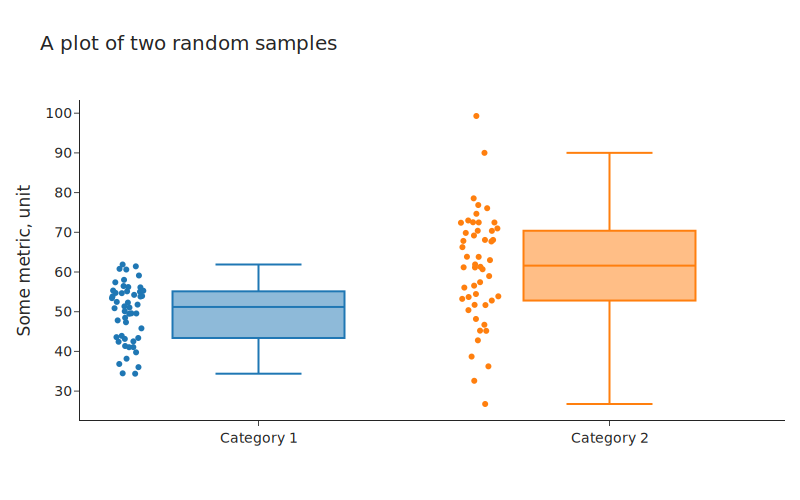
\includegraphics[width = \linewidth]{img/plt}
    \caption{Plot of two random samples.}
\end{figure}

According to the Newton's Second Law, $F=ma$, where $m$ is something\footnote{Explanation of what ``something'' means.}.

hyphen: borther-in-law

en-dash: read pages 12--36

em-dash: sldkjfsldf --- sjldfkj skldf

minus sign: $-$

\begin{equation}
    \alpha
\end{equation}


\begin{table}[htbp]
    \centering\small
    \caption{My table}
    \begin{tabular}{p{3cm}cr}
        \toprule
            \textbf{Header 1} & \textbf{Header 2} & \textbf{Header 3} \\
        \midrule
            Value 1 & Value 2 & Value 3 \\
            Value 4 & Value 5 & Value 6 \\
        \bottomrule
    \end{tabular}
    \label{tab:dummy-table}
\end{table}

sldkjfskdflsdf
